\chapter{Kilika}

\begin{enumerate}
    \item \sd\ on exiting the boat, go up and left, \sd. \skippablefmv[2:00], (press Start immediately after skip) \sd
    \item Exit inn, go right to \wakka, \sd. Go left and up to Kilika Woods, \sd
\end{enumerate}
\begin{battle}{Lancet Tutorial}
    \begin{itemize}
        \item \sd
        \kimahrif Lancet
        \switch{\kimahri}{\wakka}
        \wakkaf Defend
        \tidusf Attack
        \item \textit{If Valefor died on Sin Fin:}
        \begin{itemize}
            \switch{\lulu}{\yuna}
            \summon{\valefor}
            \valeforf Boost x2
            \valeforf Fire
        \end{itemize}
        \item \textit{Else:}
        \begin{itemize}
            \luluf Fire
        \end{itemize}
    \end{itemize}
\end{battle}
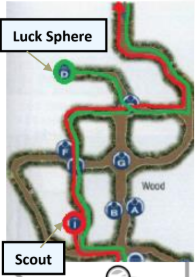
\includegraphics{graphics/kilikamap}
\begin{enumerate}[resume]
    \item Go left and up the hidden path, \pickup{Scout}
\end{enumerate}
\bothvfill\winvfill\lossvfill
\begin{spheregrid}
    \begin{itemize}
        \tidusf
        \begin{itemize}
            \item Move $\leftarrow\leftarrow$ or $\nwarrow$
            \item Flee, Agi+1 (, Str +1 if you didn't get it already)
        \end{itemize}
    \end{itemize}
    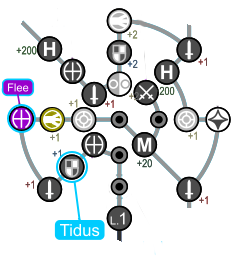
\includegraphics{graphics/Tidus_Kilika}
\end{spheregrid}
\begin{equip}
    \begin{itemize}
        \wakkaf Scout/Ice Ball
        \wakkaf Any Armguard (optional)
        \tidusf Ice Brand (optional)
    \end{itemize}
\end{equip}
\begin{enumerate}[resume]
    \item \formation{\tidus}{\wakka}{\lulu}
    \item Continue up the hidden path, following the map. Fight encounters as described below.
    \item Need 45 AP on \tidus, which is 5 kills (Overkills count as 2). This is your main source of Speed Spheres but you can obtain the rest later.
    \item You can benefit from kills beyond the first 5 but do not intentionally farm encounters and stop killing if you have 17 kills already.
\end{enumerate}
\begin{encounters}
    \begin{itemize}
        \item \textit{If there is only Ragoras:}
        \begin{itemize}
            \tidusf Flee
        \end{itemize}
        \tidusf Attack the Dinonix if present, else Defend
        \wakkaf Attack the Killer Bee if present, else Defend
        \luluf Water the Yellow Element or Killer Bee
        \tidusf Flee
    \end{itemize}
\end{encounters}
\begin{enumerate}[resume]
    \item \sd
    \item \formation{\tidus}{\yuna}{\lulu}
    \item \save
\end{enumerate}
\bothvfill\winvfill\lossvfill
\begin{battle}[3000]{Sinspawn Geneaux}
    \begin{itemize}
        \item \textit{If \tidus\ is going before \yuna:}
        \begin{itemize}
            \tidusf Defend
        \end{itemize}
        \item \textit{Else:}
        \begin{itemize}
            \switch{\yuna}{\wakka}
            \wakkaf Defend
            \tidusf Defend
            \switch{\lulu}{\yuna}
        \end{itemize}
        \summon{\valefor}
        \valeforf \od\ Energy Ray
        \valeforf Fire x3
        \valeforf \od\ Energy Ray
    \end{itemize}
    Guaranteed 4 Power Spheres, if Rare Drop from Geneaux +2 Power Spheres.
\end{battle}
\begin{enumerate}[resume]
    \item \sd\ on stone steps and temple. go into temple. Walk up to \wakka\ and Pray. \sd\ inside temple and go up steps. Wait for lift and \sd.
\end{enumerate}
\begin{trial}
    \begin{itemize}
        \item Take the sphere from the pedestal
        \item Place into the door, take it off of the door.
        \item Place sphere into the next door, take the sphere back.
        \item Place the sphere into the right holder
        \item Touch glpyh
        \item Take the sphere from the next room
        \item Place it into the left holder
        \item Take the glyph sphere from the pedestal
        \item Place it in the Fire Room
        \item Take the sphere that you put into the right holder
        \item Use it to open the door in the Fire Room
        \item Take the sphere off the door
        \item Enter the Fayth room
    \end{itemize}
\end{trial}
\begin{enumerate}[resume]
    \item In Fayth room, \sd, speak to \wakka\ first. Try to leave room, \sd, name \ifrit
    \item Hold down to exit temple, \cs[0:40], \sd
    \item \formation{\tidus}{\wakka}{\lulu}
    \item Go south through Kilika Woods, take the left path and \pickup{Luck Sphere}, referencing the above map.
    \item Exit Kilika Woods same way that you entered, treating fights the same way as above.
    \item Do the below Sphere Grid if \tidus\ has 5 S.Levels.
    \item Go down and right to S.S. Winno. \sd
\end{enumerate}